\chapter{Implementation}
\label{ch:implementation}

This chapter details the implementation of the BondHealth hospital management system, describing each module's routing logic, database interactions, and integration with the broader application. The implementation follows a layered architecture: Express.js handles HTTP routing, Neon PostgreSQL serves as the persistent store, and server-rendered EJS templates present the user interface. All code is organised within a single Node.js project, with environment-specific settings separated into a \texttt{.env} file.

% ─────────────────────────────────────────────────────────────────────────────
\section{Development Environment Setup}
\label{sec:dev-env}

The project runs on Node.js (v20 LTS) with the Express.js framework. The database is a serverless PostgreSQL instance hosted on Neon, accessed through the \texttt{@neondatabase/serverless} driver over WebSockets, requiring no persistent TCP connection pool. Sensitive configuration values — database connection strings, JWT secrets, payment gateway keys, and Socket.io settings — are stored in a \texttt{.env} file at the project root and loaded via the \texttt{dotenv} package.

\vspace{1em}
\begin{table}[ht]
\centering
\begin{tabular}{ll}
\hline
\textbf{Path} & \textbf{Purpose} \\
\hline
\texttt{/} & Project root; \texttt{package.json}, \texttt{.env}, \texttt{server.js} \\
\texttt{/routes/} & Express route files, one per role or feature domain \\
\texttt{/middleware/} & Authentication guards and role-checking middleware \\
\texttt{/views/} & EJS templates organised by role sub-folder \\
\texttt{/public/} & Static assets: CSS, client-side JS, uploaded files \\
\texttt{/db/} & Database helper and query wrapper \\
\texttt{/images/chapter5/} & Screenshots used in this chapter \\
\hline
\end{tabular}
\caption{Project Folder Structure}
\label{tab:folder-structure}
\end{table}

\noindent
The entry point \texttt{server.js} registers middleware (body parsing, cookie parsing, static files), mounts the route modules, and starts the HTTP server. Socket.io is attached to the same server instance so that WebSocket upgrade requests share the same port as REST traffic.

% ─────────────────────────────────────────────────────────────────────────────
\section{Authentication Implementation}
\label{sec:auth}

All authentication logic resides in \texttt{routes/auth.js}. Registration accepts a role parameter (\texttt{patient}, \texttt{doctor}, \texttt{admin}, or \texttt{lab}); passwords are hashed with \texttt{bcrypt} at a work factor of 12 before storage. On successful login, the server generates a signed JWT containing the user's ID, email, and role, written into an HTTP-only cookie with \texttt{Secure} and \texttt{SameSite=Strict} attributes to prevent client-side access and cross-site request forgery.

\noindent
Subsequent requests are authenticated by the \texttt{verifyToken} middleware, which reads the cookie, verifies the signature, and attaches the decoded payload to \texttt{req.user}. Role-specific guards (\texttt{requirePatient}, \texttt{requireDoctor}, \texttt{requireAdmin}, \texttt{requireLab}) wrap \texttt{verifyToken} and additionally compare \texttt{req.user.role} against the expected value, returning 403 on mismatch. The login and registration page, shown in Figure~\ref{fig:login}, presents a role selector that updates the form dynamically without a page reload.

\begin{figure}[ht]
\centering
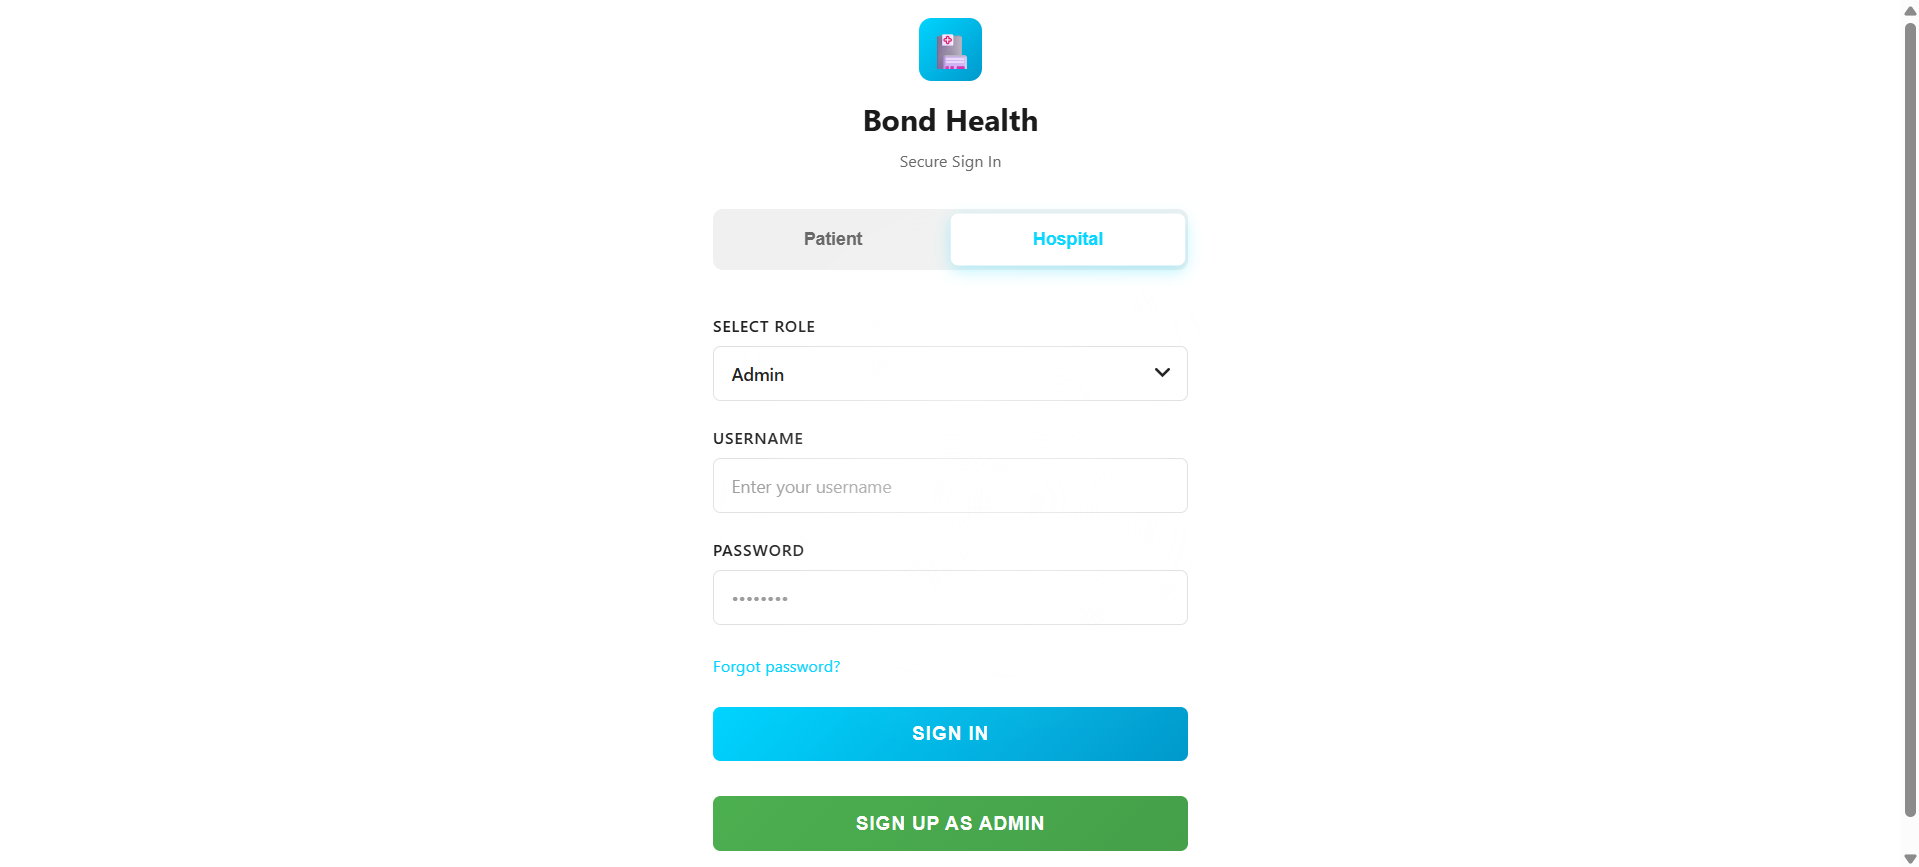
\includegraphics[width=0.85\textwidth]{images/chapter5/login-page.png}
\caption{Login and registration page with role selection.}
\label{fig:login}
\end{figure}

% ─────────────────────────────────────────────────────────────────────────────
\section{Patient Module Implementation}
\label{sec:patient}

\subsection{Patient Dashboard}
\label{subsec:patient-dashboard}

The patient dashboard is rendered server-side by the \texttt{GET /patient/dashboard} route, which executes three parallel queries: upcoming appointments (joined with doctor name and specialisation), the most recent prescription summary, and any pending lab reports. Results are passed as template variables to the EJS view, which assembles the profile summary card, appointments list, and quick action buttons. Figure~\ref{fig:dashboard-patient} shows the rendered dashboard.

\begin{figure}[ht]
\centering
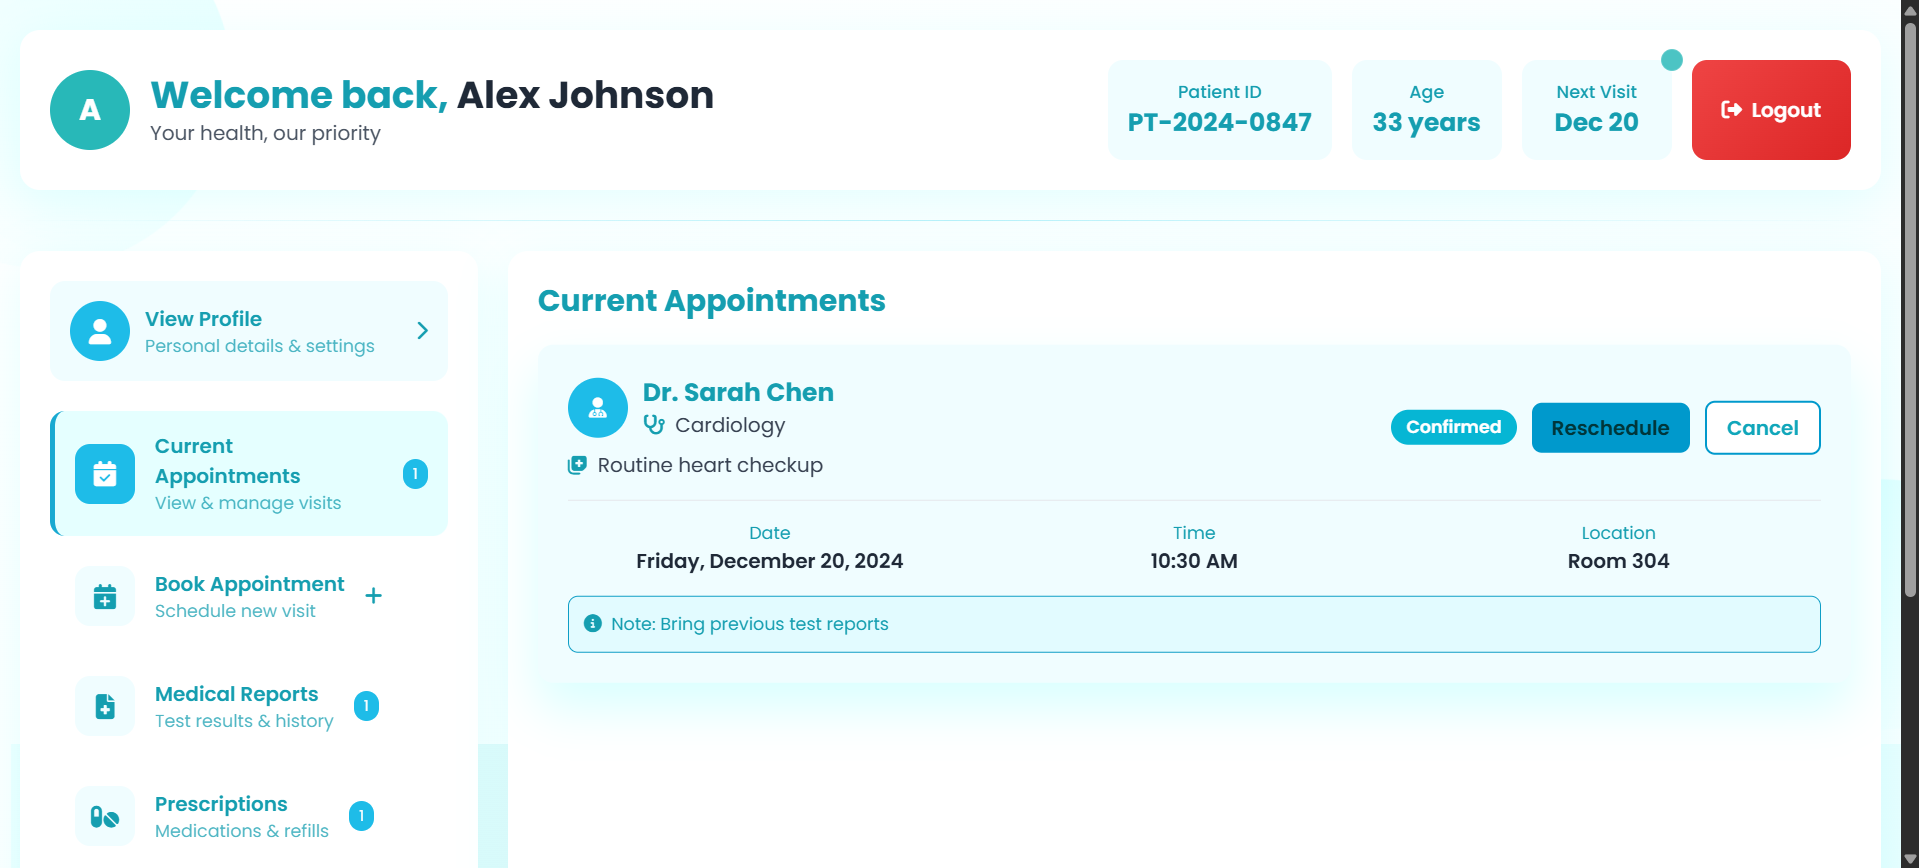
\includegraphics[width=0.85\textwidth]{images/chapter5/dashboard-patient.png}
\caption{Patient dashboard showing upcoming appointments, profile summary, and quick actions.}
\label{fig:dashboard-patient}
\end{figure}




\subsection{Appointment Booking Flow}
\label{subsec:appt-booking}

Appointment booking proceeds through three sequential steps managed by \texttt{routes/patient/appointments.js}. In Step 1, the patient submits a specialisation or name fragment queried against the \texttt{doctors} table with an \texttt{ILIKE} filter. In Step 2, the route fetches the doctor's weekly availability, subtracts already-booked slots and approved leave periods, and renders the remaining free slots as a date-and-time grid. In Step 3, the selected slot is submitted to a \texttt{POST} handler that opens a database transaction, inserts a row into \texttt{appointments} with status \texttt{pending\_payment}, and commits only after payment succeeds (see Section~\ref{sec:payment}). Figure~\ref{fig:appt-booking} shows the booking interface.

\begin{figure}[ht]
\centering
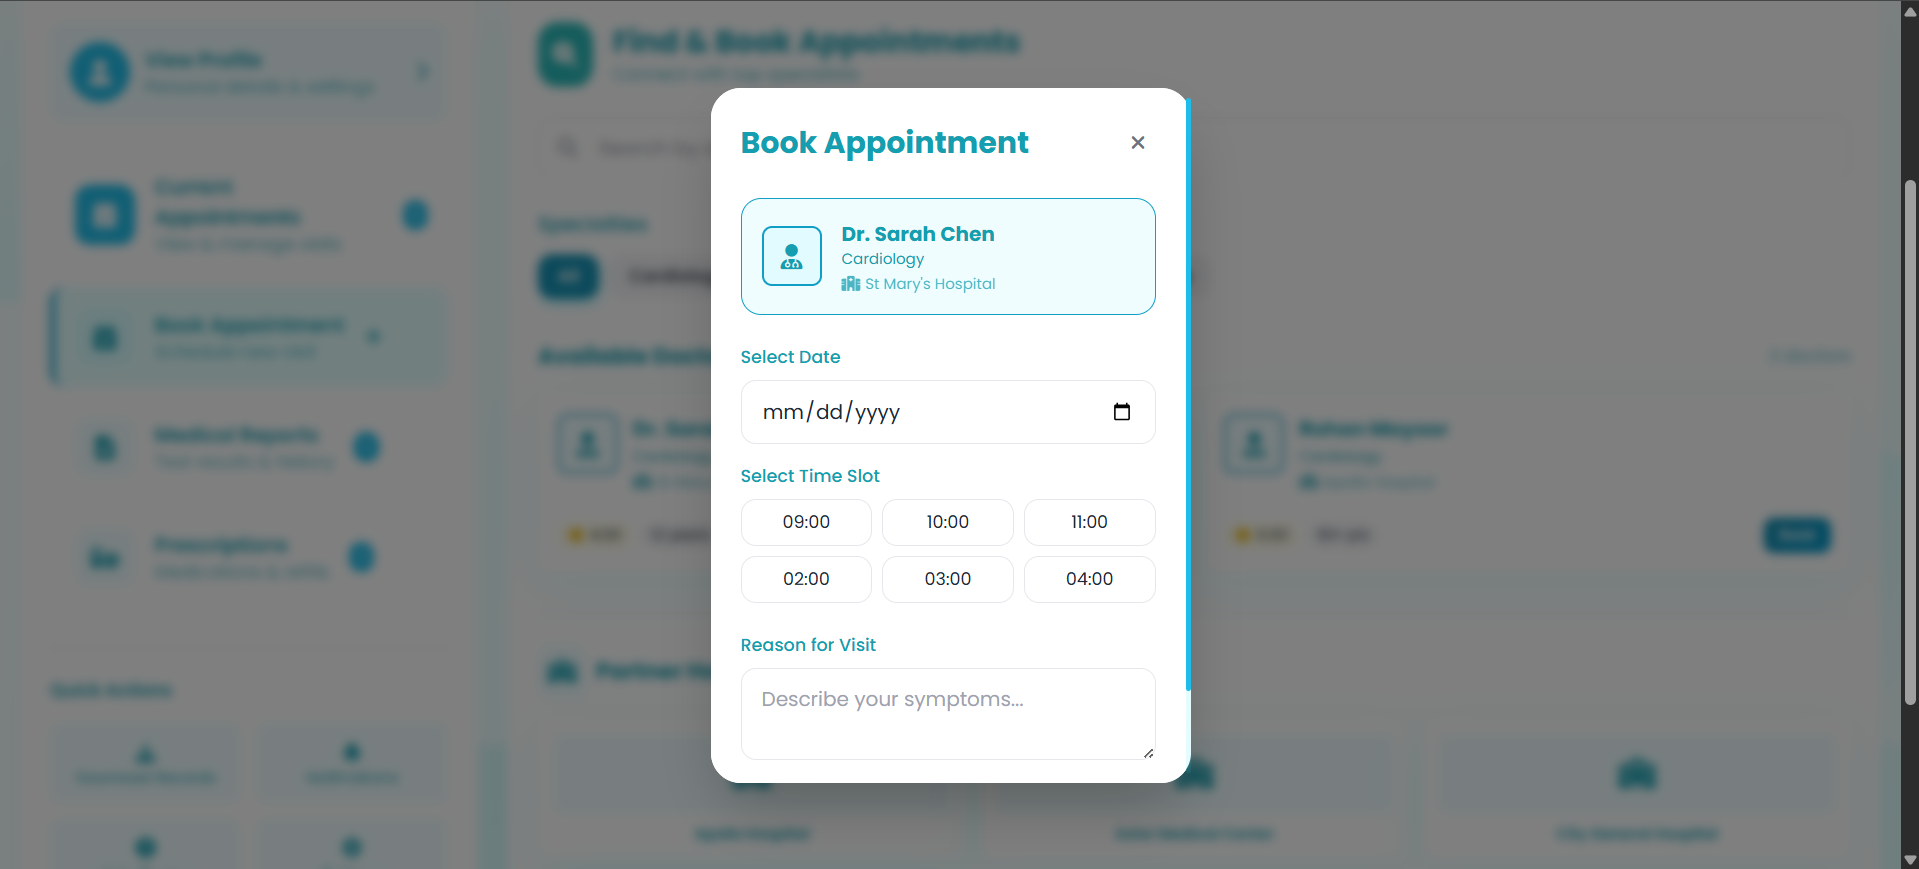
\includegraphics[width=0.85\textwidth]{images/chapter5/appointment-booking.png}
\caption{Appointment booking interface showing doctor search, time slot grid, and booking form.}
\label{fig:appt-booking}
\end{figure}

\subsection{Prescription and Lab Report Viewing}
\label{subsec:patient-records}

Prescriptions are retrieved via a join between \texttt{prescriptions}, \texttt{prescription\_items}, and \texttt{medicines}, listing each medicine with its dosage, frequency, and duration. Lab reports are retrieved from \texttt{lab\_reports} filtered by \texttt{patient\_id}; the patient can download any attached file whose \texttt{shared} flag is set to true by the lab technician.

\subsection{Profile Management}
\label{subsec:patient-profile}

The patient profile page allows updating of contact details, emergency contact, and blood group. The \texttt{POST /patient/profile} handler validates field lengths and formats, then issues an \texttt{UPDATE} on the \texttt{patients} table. Password changes require the current password to be verified with \texttt{bcrypt.compare} before the new hash is stored.

% ─────────────────────────────────────────────────────────────────────────────
\section{Doctor Module Implementation}
\label{sec:doctor}

The doctor dashboard, shown in Figure~\ref{fig:dashboard-doctor}, is rendered by \texttt{GET /doctor/dashboard}, fetching today's appointments ordered by time, the count of lab reports awaiting review, and a side-panel patient list for the current week.

\begin{figure}[ht]
\centering
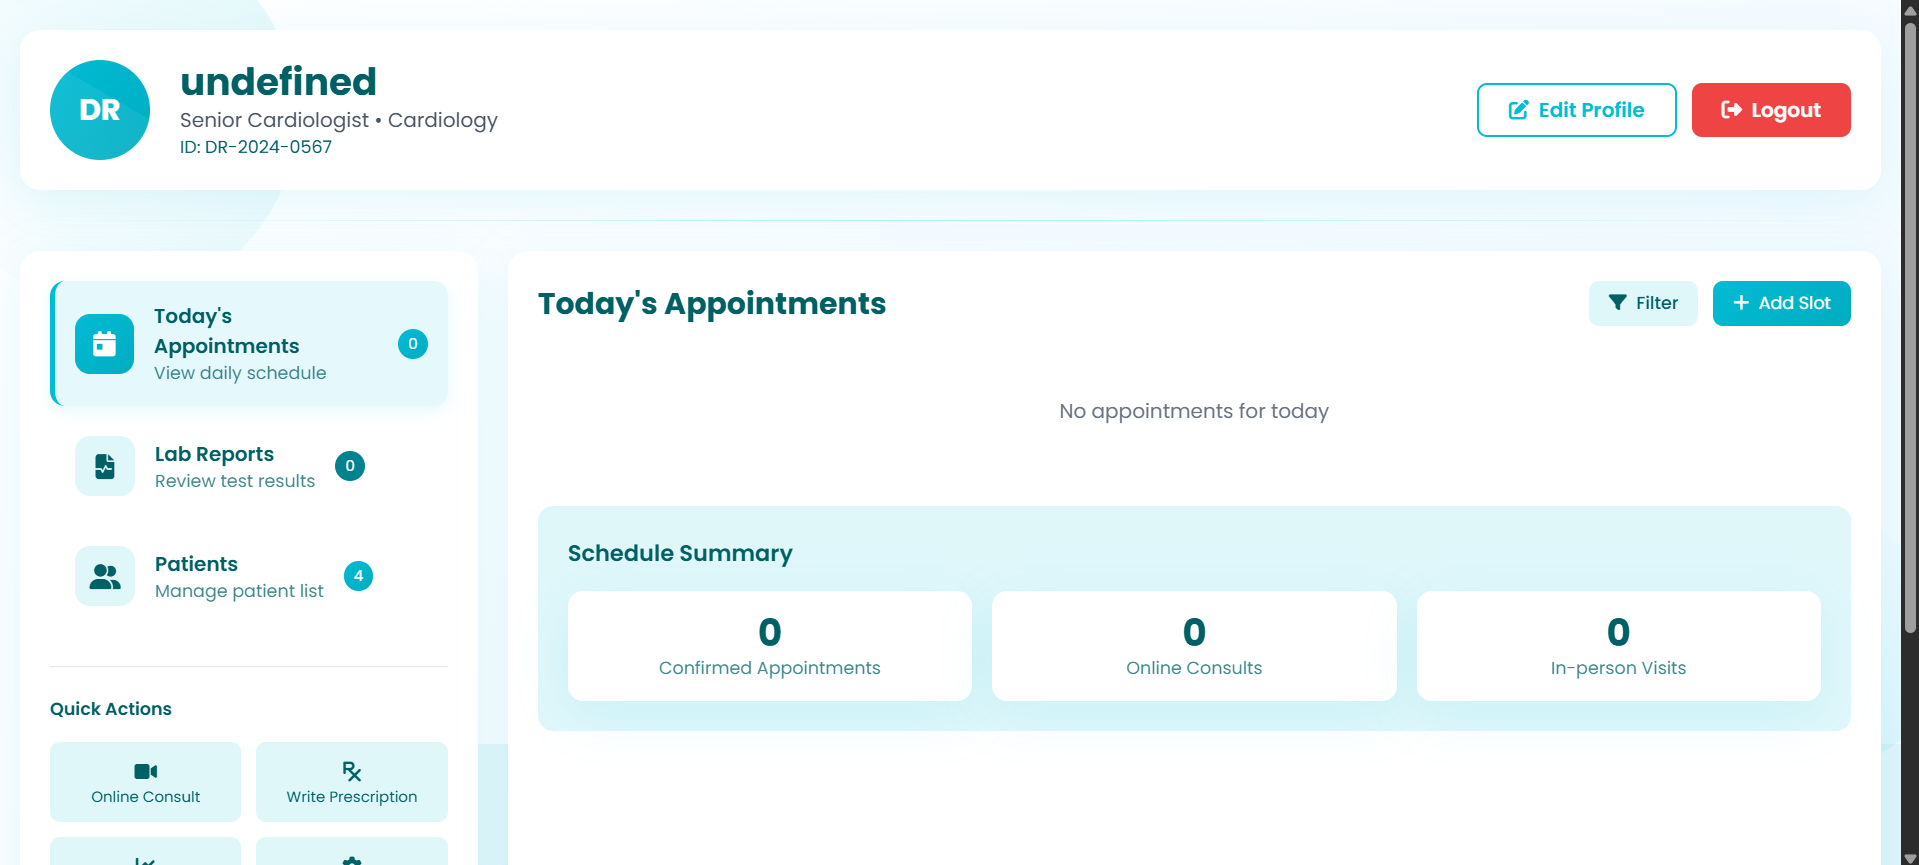
\includegraphics[width=0.85\textwidth]{images/chapter5/dashboard-doctor.png}
\caption{Doctor dashboard showing today's schedule, patient list, and lab report queue.}
\label{fig:dashboard-doctor}
\end{figure}

\subsection{Patient Consultation View}
\label{subsec:consultation}

Selecting an appointment opens the consultation view at \texttt{GET /doctor/appointment/:id}, which joins \texttt{appointments} with \texttt{patients} and loads any previous prescriptions for that patient. The doctor can add notes saved to the \texttt{appointments.doctor\_notes} column.

\subsection{Prescription Writing}
\label{subsec:prescription}

The prescription form submits to \texttt{POST /doctor/prescription}, which inserts a row into \texttt{prescriptions} and iterates over the submitted medicine array, inserting one row per medicine into \texttt{prescription\_items}. Both inserts run inside a single transaction to prevent orphaned prescription headers on partial failure.

\subsection{Lab Report Review}
\label{subsec:lab-review}

Reports shared with the doctor are retrieved from \texttt{lab\_reports} filtered by \texttt{doctor\_id}, rendering the test name, result value, reference range, and any attached file. The doctor can mark a report as reviewed, setting \texttt{lab\_reports.reviewed\_by\_doctor} to true.

\subsection{Leave Application}
\label{subsec:leave}

The leave application form collects start date, end date, and reason. On submission, \texttt{POST /doctor/leave} inserts a row into \texttt{doctor\_leaves} with status \texttt{pending}, after which the availability query excludes any slots overlapping with approved leave for that doctor.

% ─────────────────────────────────────────────────────────────────────────────
\section{Admin Module Implementation}
\label{sec:admin}

The admin dashboard, shown in Figure~\ref{fig:dashboard-admin}, aggregates hospital-wide statistics through parallel \texttt{COUNT} and \texttt{SUM} queries: total registered patients, active doctors, appointments in the current month, and medicines below their reorder threshold.

\begin{figure}[ht]
\centering
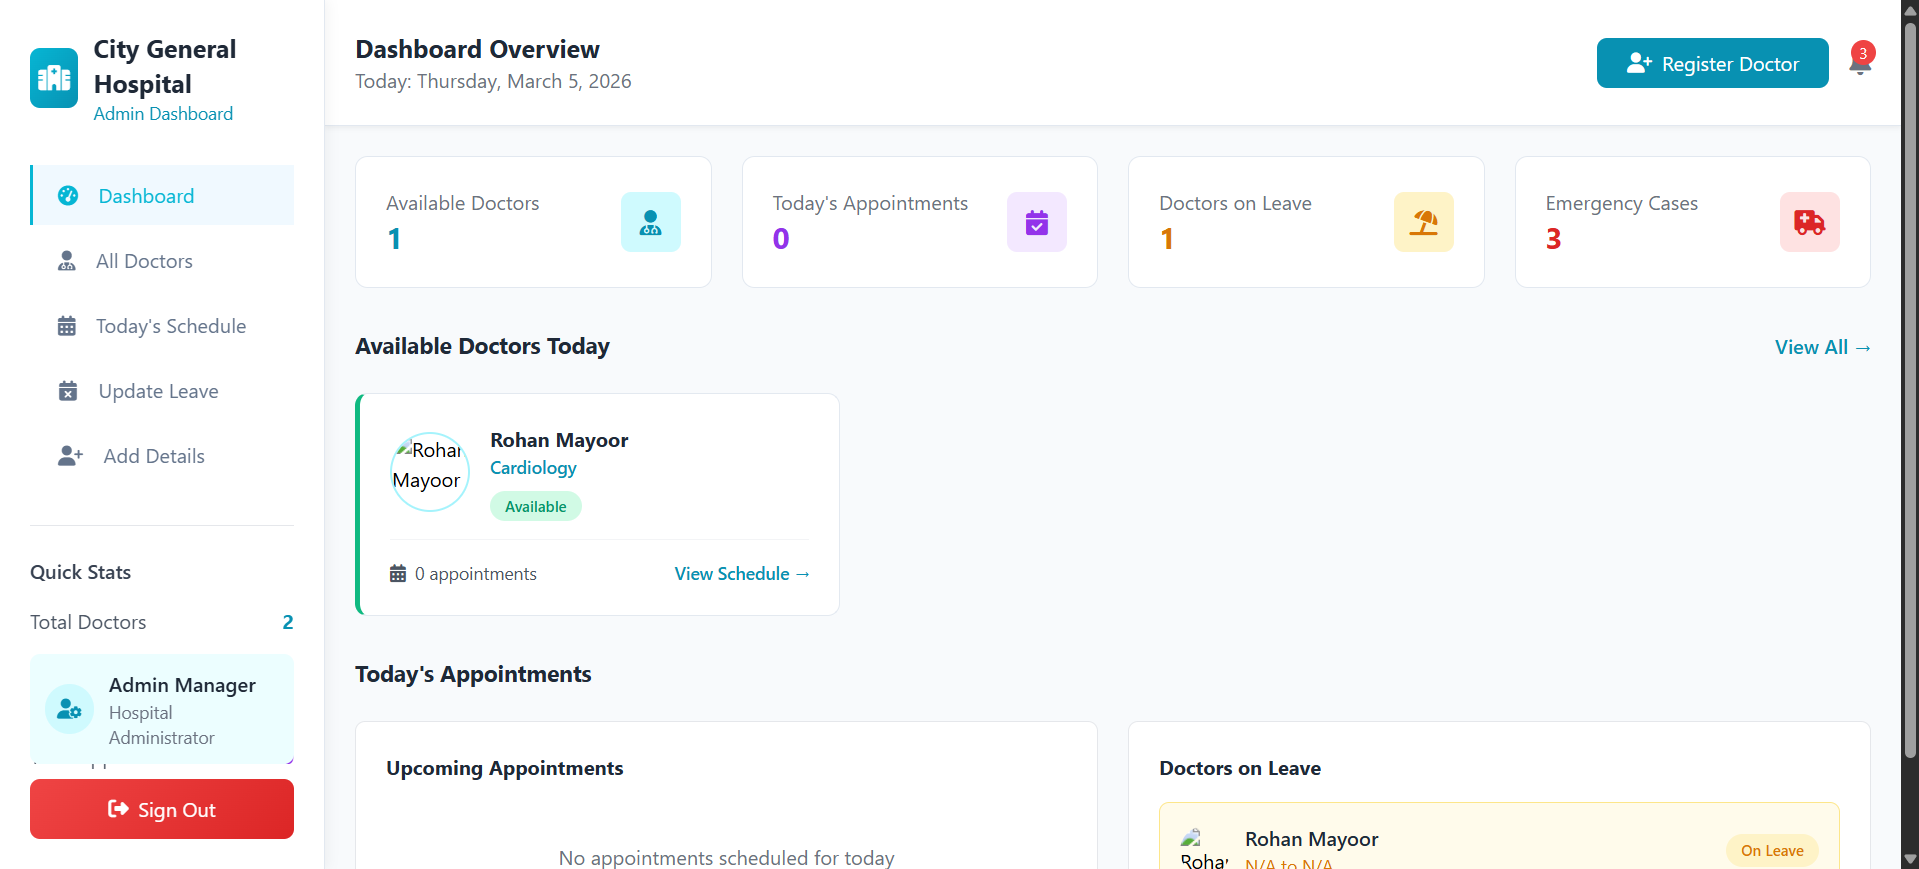
\includegraphics[width=0.85\textwidth]{images/chapter5/dashboard-admin.png}
\caption{Admin dashboard with statistics cards and management panels.}
\label{fig:dashboard-admin}
\end{figure}

\subsection{Doctor Registration}
\label{subsec:admin-doctor}

Doctors are registered at \texttt{POST /admin/doctors/create}. The handler hashes the initial password, inserts into \texttt{users} with role \texttt{doctor}, then inserts the profile row into \texttt{doctors} (specialisation, qualification, consultation fee). Both inserts are wrapped in a transaction to prevent a \texttt{users} row existing without a corresponding \texttt{doctors} profile.

\subsection{Medicine Inventory Management}
\label{subsec:medicine}

The medicine management page lists all rows from the \texttt{medicines} table with current stock and reorder level. Admins can add medicines, update stock via parameterised \texttt{UPDATE} statements, and deactivate discontinued medicines by setting an \texttt{is\_active} flag rather than deleting rows, preserving referential integrity with historical prescriptions.

\subsection{Lab Technician Account Creation}
\label{subsec:lab-account}

Lab technician accounts are created at \texttt{POST /admin/lab/create}, following the same two-table pattern as doctor registration: an entry in \texttt{users} with role \texttt{lab} and a supplementary row in \texttt{lab\_technicians}.

\subsection{Leave Approval Workflow}
\label{subsec:leave-approval}

The admin views pending leave requests from \texttt{doctor\_leaves} where \texttt{status = 'pending'}. Approving issues an \texttt{UPDATE} to \texttt{status = 'approved'}, causing the availability query to exclude those dates. Rejecting sets \texttt{status = 'rejected'} and optionally stores a rejection reason.

% ─────────────────────────────────────────────────────────────────────────────
\subsection{Lab Technician Module Implementation}

\subsubsection{Report Submission Form}

The report submission interface, shown in Figure 5.6, is rendered by \texttt{GET /lab/report/new}. It walks the technician through a structured multi-step process on a single page, with each step validated before the next becomes accessible.

\begin{enumerate}
    \item \textbf{Patient Selection} — A search field queries registered patients by name or patient ID in real time, populating a dropdown with matching results and displaying basic patient details as a confirmation prompt.

    \item \textbf{Test Entry} — The technician selects or types the test name from a pre-populated, hospital-scoped list of diagnostic tests, then enters the result value and reference range into dedicated fields.

    \item \textbf{Result Validation} — Client-side logic immediately compares the entered result against the reference range and flags out-of-range values with a visual indicator, serving as a safeguard against data entry errors without blocking submission.

    \item \textbf{File Upload} — An optional PDF or image of the physical report can be attached. The file is validated for type and size client-side, saved server-side to \texttt{/public/uploads/reports/}, and its path stored in \texttt{lab\_reports.file\_path}.

    \item \textbf{Sharing Preferences} — Checkboxes determine visibility: the technician can share the report with the patient, the referring doctor, or both. Selections map directly to the corresponding boolean columns in the \texttt{lab\_reports} table.
\end{enumerate}

On submission, a \texttt{POST} request is dispatched to \texttt{/lab/report/submit}, which validates the payload server-side, persists the record, and redirects the technician to the report list view where the new entry appears at the top with a timestamp and patient reference.

\begin{figure}[ht]
\centering
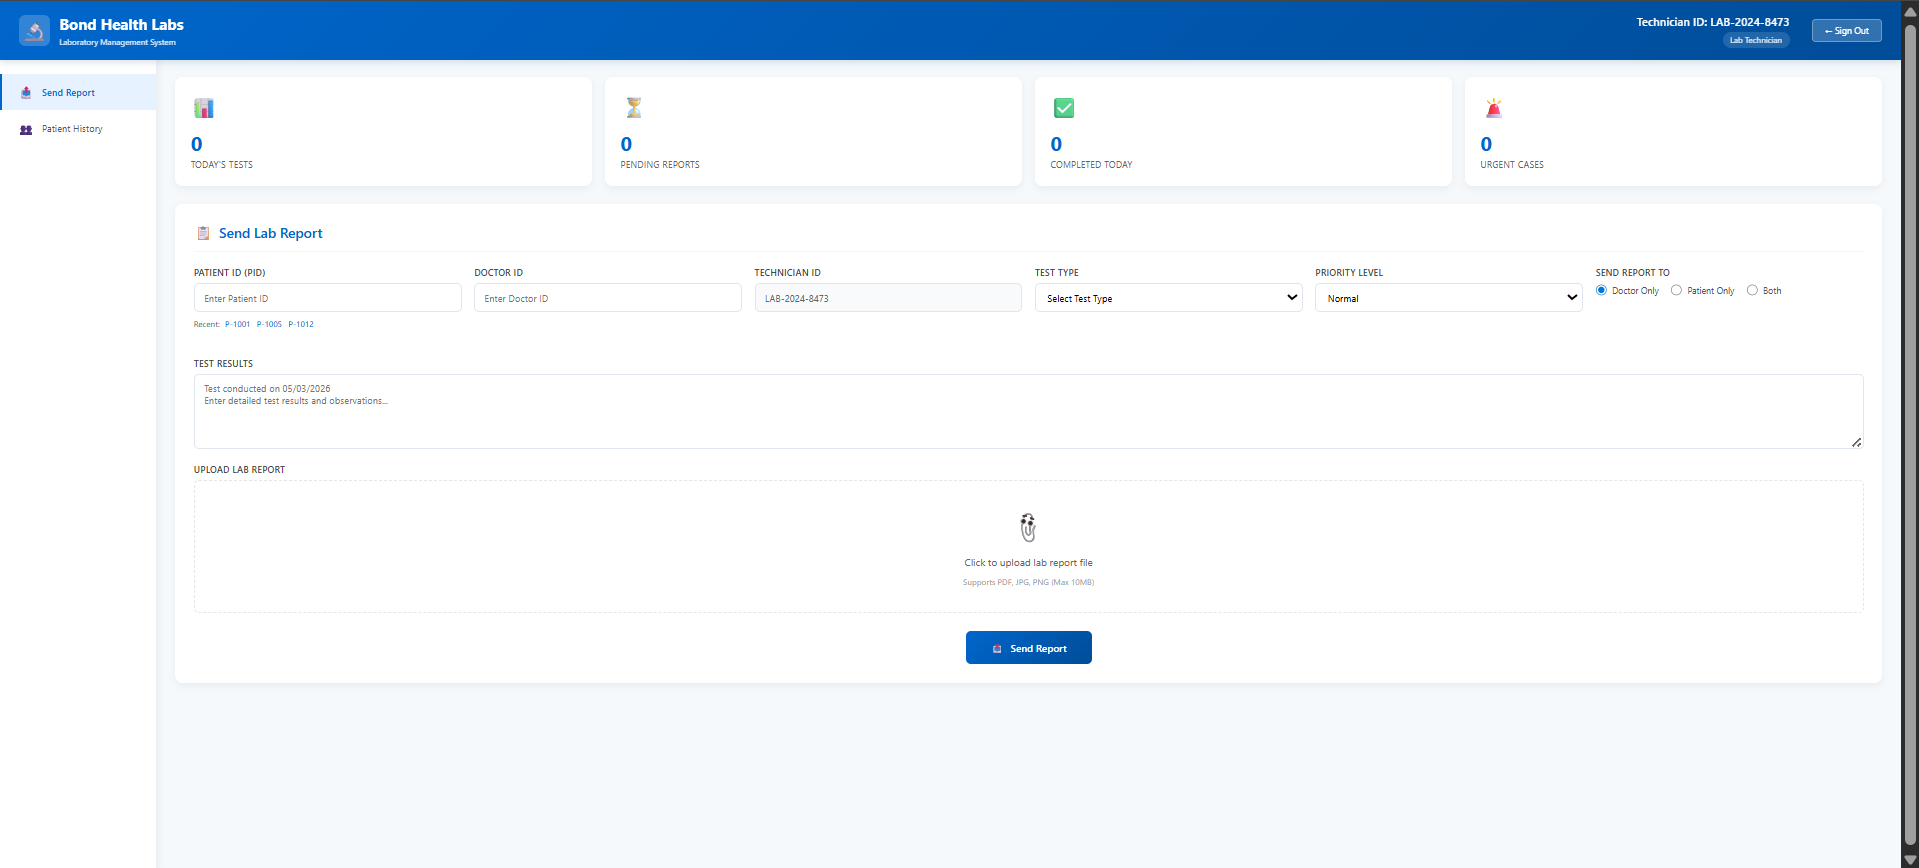
\includegraphics[width=0.85\textwidth]{images/chapter5/lab-report-form.png}
\caption{Lab technician report submission form with patient selection and result entry.}
\label{fig:lab-form}
\end{figure}

\subsection{Patient History Table}
\label{subsec:lab-history}

Below the submission form, the technician's home page renders a paginated table of previously submitted reports ordered by submission date descending. Each row shows the patient name, test name, submission date, and current sharing status, with an edit link for correction within a configurable time window.

% ─────────────────────────────────────────────────────────────────────────────
\section{Payment Implementation}
\label{sec:payment}

Payment processing is integrated at \texttt{routes/payment.js}. When a patient confirms a slot (Section~\ref{subsec:appt-booking}), the handler creates a payment intent via the gateway API using the fee from \texttt{doctors.consultation\_fee}. The returned client secret is passed to the EJS template, where client-side JavaScript mounts the payment widget without card details touching the application server.

\noindent
On successful authorisation, the gateway sends an asynchronous webhook \texttt{POST} to \texttt{/payment/webhook}. The handler verifies the event signature using the gateway's signing secret, then updates the \texttt{appointments} row from \texttt{pending\_payment} to \texttt{confirmed}. Webhook-driven confirmation ensures appointment status is always set by an authoritative server-to-server event, even if the patient closes the browser after payment.

% ─────────────────────────────────────────────────────────────────────────────
\section{Real-Time Messaging Implementation}
\label{sec:messaging}

Real-time chat is implemented with Socket.io attached to the Express HTTP server. When a user opens the messaging view, the client emits a \texttt{joinRoom} event carrying the appointment ID; the server places the socket into a named room derived from that ID, isolating messages per consultation.

\noindent
Incoming \texttt{sendMessage} events are persisted to the \texttt{messages} table — capturing sender ID, room ID, content, and timestamp — before broadcasting a \texttt{receiveMessage} event to the room. Persisting before broadcasting allows reconnecting users to retrieve full conversation history from the database on page load, independent of Socket.io's in-memory state. A Redis adapter shares the room registry across server instances, enabling horizontal scaling.

% ─────────────────────────────────────────────────────────────────────────────
\section{Database Query Implementation}
\label{sec:db-queries}

All database access goes through a thin helper in \texttt{db/index.js} exposing a single \texttt{query(sql, params)} function. Parameterised placeholders (\texttt{\$1}, \texttt{\$2}, \ldots) are used throughout to prevent SQL injection.

\subsection{Availability Check}
\label{subsec:avail-query}

The availability query returns only slots satisfying all three conditions simultaneously: the slot falls within the doctor's declared availability for that weekday, no confirmed appointment occupies it, and the date does not overlap with any approved leave. A \texttt{LEFT JOIN} from the generated slot series against \texttt{appointments} and \texttt{doctor\_leaves} filters where both join targets return \texttt{NULL}.

\subsection{Appointment Creation with Transaction}
\label{subsec:appt-transaction}

Appointment insertion is wrapped in an explicit transaction to guard against double-booking under concurrent requests. The transaction locks the target slot with \texttt{SELECT \ldots FOR UPDATE}, rechecks availability within the lock, inserts the appointment, and commits. If the recheck finds the slot taken, the transaction rolls back and the route returns a conflict response.

\subsection{UUID Generation}
\label{subsec:uuid}

Primary keys for \texttt{users}, \texttt{appointments}, \texttt{prescriptions}, and \texttt{lab\_reports} use UUIDs generated by PostgreSQL's \texttt{gen\_random\_uuid()} function as a column default, avoiding guessable sequential IDs in URLs and removing the need for application-level UUID libraries.

\subsection{Index Usage}
\label{subsec:indexes}

Indexes are defined on columns most frequently used in \texttt{WHERE} clauses: \texttt{appointments.patient\_id}, \texttt{appointments.doctor\_id}, \texttt{appointments.appointment\_date}, \texttt{lab\_reports.patient\_id}, and \texttt{doctor\_leaves.doctor\_id}. These allow dashboard and availability queries to use index scans rather than sequential scans as the dataset grows.

% ─────────────────────────────────────────────────────────────────────────────
\section{Summary}
\label{sec:implementation-summary}

This chapter has presented the implementation of each module within the BondHealth platform. From the authentication layer through to the real-time messaging system, every component has been built with consistent emphasis on security, data integrity, and maintainability. The layered architecture separating routing, business logic, and database access ensures each module remains independently testable and extensible. Parameterised queries, transactional inserts, and webhook-driven payment confirmation collectively reflect a production-grade approach to healthcare application development. The following chapter details the testing strategy employed to validate the correctness and robustness of the implementation described here.